\documentclass[border=4pt,12pt]{standalone}
% House style for redrawn exam diagrams (diagram-v4: 0.4pt lines, filled -latex arrows, fine dashes; stipple and hatching drawn as real dots/lines (no PDF/SVG patterns, so they render in every browser and at any scale); transparent background). Every figure \input's this.
\usepackage{amsmath,amssymb}
\usepackage{txfonts}
\usepackage{pdfrender,xcolor}
% \halo{text}: label on shading. The shading stops just around each letter's outline (a thin knock-out that follows the
% glyphs, like the papers' typesetting), never a box. Owner: "I don't want a box around the text".
\newcommand{\halo}[1]{\leavevmode\rlap{\pdfrender{TextRenderingMode=2,LineWidth=2.2pt,LineJoinStyle=1,StrokeColor=white,FillColor=white}#1}#1}
\usepackage{tikz,pgfplots}
\pgfplotsset{compat=1.18}
\usetikzlibrary{arrows.meta,calc,angles,quotes,patterns,patterns.meta,intersections,positioning,decorations.markings,shapes.geometric}
% Stipple and hatching are drawn as actual dots / lines clipped to the region (path picture), NOT as pattern fills:
% SVG <pattern> fills vanish or blur when browsers scale the image, so the owner could not see the shading.
% Each dot is a 0.72pt square (keeps SVGs small; reads as a dot at print size). Dots sit on one global staggered grid, so neighbouring regions line up.
\makeatletter
\newdimen\ex@x \newdimen\ex@y \newdimen\ex@xa \newdimen\ex@ya \newdimen\ex@xb \newdimen\ex@yb \newcount\ex@row
\def\exam@stipplecolor{black!75}\def\exam@dotr{0.42pt}\def\exam@dotgap{2.5}
\def\ex@rowdots{\ifdim\ex@x<\ex@xb \pgfpathrectangle{\pgfqpoint{\dimexpr\ex@x-0.36pt\relax}{\dimexpr\ex@y-0.36pt\relax}}{\pgfqpoint{0.72pt}{0.72pt}}\advance\ex@x by \exam@dotgap pt\relax\expandafter\ex@rowdots\fi}
\def\exam@stipple{%
  \pgftransformreset% dots are sized in real points even inside scaled pictures
  \pgfpointanchor{path picture bounding box}{south west}\ex@xa=\pgf@x \ex@ya=\pgf@y
  \pgfpointanchor{path picture bounding box}{north east}\ex@xb=\pgf@x \ex@yb=\pgf@y
  \pgfsetfillcolor{\exam@stipplecolor}\pgfmathsetmacro\ex@h{\exam@dotgap/2}%
  \pgfmathtruncatemacro\ex@r{floor(\ex@ya/\ex@h)-1}\ex@row=\ex@r\relax
  \ex@y=\ex@r\dimexpr\ex@h pt\relax
  \loop\ifdim\ex@y<\ex@yb
    \pgfmathtruncatemacro\ex@c{floor(\ex@xa/\exam@dotgap)-1}\ex@x=\ex@c\dimexpr\exam@dotgap pt\relax
    \ifodd\ex@row \advance\ex@x by \ex@h pt\fi
    \ex@rowdots
    \advance\ex@y by \ex@h pt \advance\ex@row by 1
    \ifnum\numexpr\ex@row-(\ex@row/4)*4\relax=0 \pgfusepath{fill}\fi% flush every 4 rows: bounded TeX memory, few clip copies in the SVG
  \repeat\pgfusepath{fill}}
\newdimen\ex@d
\def\exam@hatch#1{% #1 = 1 for /, -1 for \ ; lines 45 degrees, 3pt apart
  \pgftransformreset
  \pgfpointanchor{path picture bounding box}{south west}\ex@xa=\pgf@x \ex@ya=\pgf@y
  \pgfpointanchor{path picture bounding box}{north east}\ex@xb=\pgf@x \ex@yb=\pgf@y
  \ex@d=\dimexpr\ex@yb-\ex@ya\relax \ex@x=\dimexpr\ex@xa-\ex@d\relax
  \loop\ifdim\ex@x<\ex@xb
    \ifnum#1>0 \pgfpathmoveto{\pgfqpoint{\ex@x}{\ex@ya}}\pgfpathlineto{\pgfqpoint{\dimexpr\ex@x+\ex@d\relax}{\ex@yb}}%
    \else \pgfpathmoveto{\pgfqpoint{\ex@x}{\ex@yb}}\pgfpathlineto{\pgfqpoint{\dimexpr\ex@x+\ex@d\relax}{\ex@ya}}\fi
    \advance\ex@x by 4.24pt
  \repeat
  \pgfsetlinewidth{0.4pt}\pgfsetstrokecolor{black}\pgfusepath{stroke}}
\def\examstipple{\exam@stipple}\def\examhatch{\exam@hatch}\def\examsetstipplecolor#1{\def\exam@stipplecolor{#1}}\def\examsetdotgap#1{\def\exam@dotgap{#1}}
\makeatother
% (legacy pattern kept for old files)
% staggered stipple like the NESA papers' dotted shading
\pgfdeclarepatternformonly{exam stipple}{\pgfpointorigin}{\pgfqpoint{2.2pt}{2.2pt}}{\pgfqpoint{2.2pt}{2.2pt}}{%
  \pgfpathcircle{\pgfqpoint{0.55pt}{0.55pt}}{0.42pt}\pgfpathcircle{\pgfqpoint{1.65pt}{1.65pt}}{0.42pt}\pgfusepath{fill}}
\tikzset{
  every picture/.style={line width=0.6pt, >={Latex[length=2mm,width=1.3mm]}},
  curve/.style={line width=0.6pt},
  open arrow/.style={-{Latex[length=2mm,width=1.3mm]}},  % owner: filled -latex heads everywhere, no open chevrons
  aux/.style={dash pattern=on 2pt off 1.5pt, line width=0.6pt},
  shade/.code={\def\exA{#1}\def\exB{none}\ifx\exA\exB\else\pgfkeysalso{fill=black!18}\fi},
  shade/.default=on,
  shade dots/.style={fill=none, path picture={\examstipple}},
  stipple color/.code={\examsetstipplecolor{#1}},
  stipple gap/.code={\examsetdotgap{#1}},
  shade dense dots/.style={fill=none, stipple gap=1.6, path picture={\examstipple}},
  shade hatch/.style={fill=none, path picture={\examhatch{1}}},
  shade hatch reverse/.style={fill=none, path picture={\examhatch{-1}}},
  shade solid/.style={fill=black},
  pt/.style={circle, fill, inner sep=1.1pt},
  open pt/.style={circle, draw, fill=white, inner sep=1.1pt},
}
\pgfplotsset{
  exam axes/.style={axis lines=middle, axis line style={->}, xlabel={$x$}, ylabel={$y$},
    xlabel style={anchor=west}, ylabel style={anchor=south}, tick label style={font=\small},
    every axis plot/.append style={line width=0.6pt, black}, samples=200, clip=false,
    enlargelimits=false, axis on top},
}

\begin{document}
% 2025 Hunters Hill AT4 Q21 solution: y=-3/x+4 with asymptotes and x-intercept annotated (crop pixels, y down)
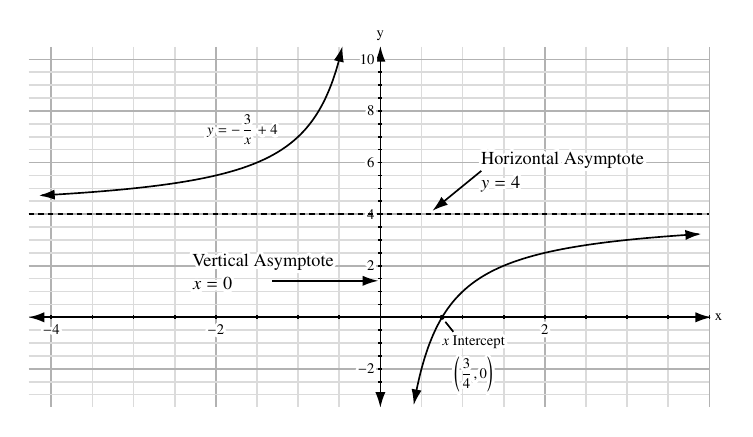
\begin{tikzpicture}[x=0.0127cm,y=-0.0127cm,font=\fontsize{5.3}{6.4}\selectfont]
  \def\ox{366}\def\oy{300.5}\def\ux{82.3}\def\uy{25.8}
  % grid: x every 0.5, y every 0.5; darker every 2
  \foreach \i in {-8,...,8}{\pgfmathsetmacro\xx{\ox+\ux*\i/2}\pgfmathsetmacro\cc{mod(abs(\i),4)==0?30:14}
    \draw[black!\cc] (\xx,30) -- (\xx,390);}
  \foreach \j in {-6,...,20}{\pgfmathsetmacro\yy{\oy-\uy*\j/2}\pgfmathsetmacro\cc{mod(abs(\j),4)==0?30:14}
    \draw[black!\cc] (14,\yy) -- (695,\yy);}
  % axes
  \draw[<->] (14,\oy) -- (697,\oy);
  \draw[<->] (\ox,391) -- (\ox,29);
  \node[anchor=west,inner sep=1pt] at (697,\oy) {x};
  \node[anchor=south,inner sep=1pt] at (\ox,27) {y};
  \foreach \i in {-8,...,8}{\pgfmathsetmacro\xx{\ox+\ux*\i/2}\draw (\xx,\oy-2) -- (\xx,\oy+2);}
  \foreach \j in {-6,...,20}{\pgfmathsetmacro\yy{\oy-\uy*\j/2}\draw (\ox-2,\yy) -- (\ox+2,\yy);}
  \foreach \v in {-4,-2,2}{\node[anchor=north,inner sep=0pt] at ({\ox+\ux*\v},307) {\halo{$\v$}};}
  \foreach \v in {10,8,6,4,2,-2}{\node[anchor=east,inner sep=0pt] at (361,{\oy-\uy*\v}) {\halo{$\v$}};}
  % asymptote y=4
  \draw[aux] (14,{\oy-4*\uy}) -- (695,{\oy-4*\uy});
  % curve
  \draw[<->,smooth] plot[domain=-4.15:-0.46,samples=90] ({\ox+\ux*\x},{\oy-\uy*(4-3/\x)});
  \draw[<->,smooth] plot[domain=0.405:3.9,samples=90] ({\ox+\ux*\x},{\oy-\uy*(4-3/\x)});
  \fill ({\ox+\ux*0.75},\oy) circle (2.5);
  % annotations
  \node at (228,113) {\halo{$y=-\dfrac{3}{x}+4$}};
  \node[anchor=west,inner sep=0pt,font=\fontsize{6.6}{8.6}\selectfont,align=left] at (466,155) {\halo{Horizontal Asymptote}\\\halo{$y=4$}};
  \draw[->] (467,154) -- (418,194);
  \node[anchor=west,inner sep=0pt,font=\fontsize{6.6}{8.6}\selectfont,align=left] at (177,255) {\halo{Vertical Asymptote}\\\halo{$x=0$}};
  \draw[->] (258,264) -- (364,264);
  \node[anchor=north,inner sep=0pt,align=center] at (459,318) {\halo{$x$ Intercept}\\[2pt]\halo{$\left(\dfrac{3}{4},0\right)$}};
  \draw (431,305) -- (439,315);
\end{tikzpicture}
\end{document}
